\documentclass[a4paper,11pt]{report}
\usepackage[T1]{fontenc}
\usepackage[utf8]{inputenc}
\usepackage{lmodern}
\usepackage{array}
\usepackage{color}
\usepackage{listings} 

% configure graphics
\usepackage{float}
\usepackage{graphicx}
\graphicspath{{images/}} % Path Where images reside
\DeclareGraphicsExtensions{.pdf,.jpeg,.png,.jpg,.png} % Valide image format extensions

% define color fot the code
\definecolor{colKeys}{rgb}{0,0,1} 
\definecolor{colIdentifier}{rgb}{0,0,0} 
\definecolor{colComments}{rgb}{0,1,0} 
\definecolor{colString}{rgb}{0.6,0.1,0.1} 

%configuration de listings pour le code
\lstset{
float=hbp,% 
basicstyle=\ttfamily\small, % 
identifierstyle=\color{colIdentifier}, % 
keywordstyle=\color{colKeys}, % 
stringstyle=\color{colString}, % 
commentstyle=\color{colComments}, % 
columns=flexible, % 
tabsize=2, % 
frame=trBL, % 
frameround=tttt, % 
extendedchars=true, % 
showspaces=false, % 
showstringspaces=false, % 
numbers=left, % 
numberstyle=\tiny, % 
breaklines=true, % 
breakautoindent=true, % 
captionpos=b,% 
xrightmargin=0.5cm, % 
xleftmargin=0.5cm 
} 

\title{Ranger User Manual}
\author{David Mansolino}

\begin{document}

\maketitle
\tableofcontents

%\begin{abstract}
%\end{abstract}






\part{Simulation}
\chapter{The model}
A Webots\footnote{http://www.cyberbotics.com/overview} simulation model of the Ranger has been created.\\

\begin{figure}[H]
  \begin{center}
    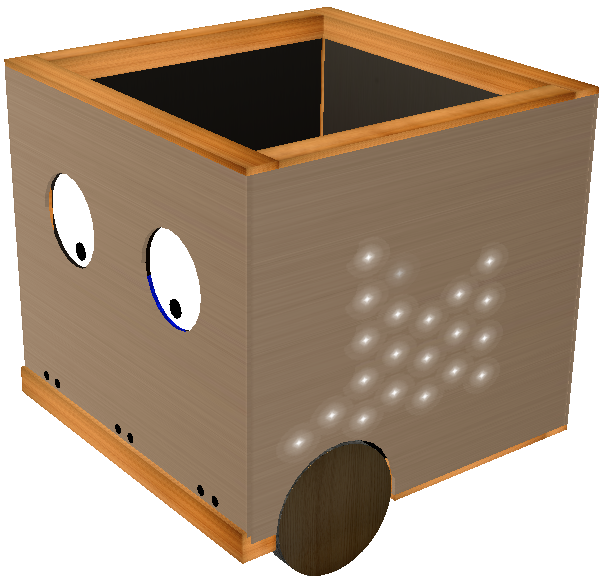
\includegraphics[width=8cm]{simulation_model.png}
    \caption{Simulation model of the ranger in Webots}
    \label{fig:simulation_model}
  \end{center}
\end{figure}

Thanks to this model and Webots, the Ranger (or even several Rangers) can easily be simulated and programmed for various type of virtual environments and conditions.\\

\section{Presentation and caracteristics of the model}
The model of the ranger robot is based on a differential wheels, and contains most of the actuators and sensors of the real Ranger robot. It also have a realistic physics: friction, dynamics and collision has been made as close from the real robot has possible.\\

\paragraph{DistanceSensors} The model contains five \textit{DistanceSensors}, three in front of the robot and two for the ground. They are respectively called: \textcolor{blue}{“dsBottomRight”}, \textcolor{blue}{“dsBottomLeft”}, \textcolor{blue}{“dsFrontRight”}, \textcolor{blue}{“dsFrontCenter”} and \textcolor{blue}{“dsFrontLeft”}.

\paragraph{TouchSensors} The model contains two \textit{TouchSensors} one bumper (called \textcolor{blue}{“bumper”}) and one force sensors for the content of the box (called \textcolor{blue}{“balance”}).

\paragraph{Accelerometer} The model contains an accelerometer (called \textcolor{blue}{“accelerometer”}).

\paragraph{Motors} The model contains heigt motors, two for each eyes and two for each eyelids. They are respectively called: \textcolor{blue}{“LeftUpperEyelid”}, \textcolor{blue}{“LeftLowerEyelid”}, \textcolor{blue}{“RightUpperEyelid”},\textcolor{blue}{“RightLowerEyelid”}, \textcolor{blue}{“leftPupilVert”}, \textcolor{blue}{“leftPupilHori”}, \textcolor{blue}{“rightPupilVert”} and \textcolor{blue}{“rightPupilHori”}. Concerning the eyelids, there range is between angle 0 (eye closed) and 0.78 (eye open) and for the pupil, the range is between -0.028 and 0.028 (0 been the center).

\paragraph{Communication} The model contains a pair of \textit{Emitter}-\textit{Receiver} of radio type (called \textcolor{blue}{“radioEmitter”} and \textcolor{blue}{“radioReceiver”}), their respective channel can be set thanks to the fields \textit{radioEmitterChannel} and \textit{radioReceiverChannel} of simulation model.

\paragraph{Range-Bearing} The model contains a range-bearing based on a pair of \textit{Emitter}-\textit{Receiver} of infrared type. They are called \textcolor{blue}{“infraredEmitter”} and \textcolor{blue}{“infraredReceiver”} and are booth using channel 1. The range and noise can be set with the fields \textit{infraredEmitterRange}, \textit{infraredEmitterSignalStrengthNoise} and \textit{infraredEmitterDirectionNoise}.

\paragraph{Display} The model contains three \textit{Displays} (\textcolor{blue}{“displayRight”}, \textcolor{blue}{“displayLeft”} and \textcolor{blue}{“displayBack”}) of resolution 256x256 in order to mimic the Leds pannels in a realistic and efficient way.

\paragraph{Extension} Finally the model contains one extension slot used to add other devices or optional components to the simulation model of the Ranger.

\paragraph{Friction} If needed a specific friction coefficient can be set for the wheels only. In order to do this, a new \textit{contactProperty} has to be added in the \textit{WorldInfo} node of the simulation. This \textit{contactProperty} need to be defined between \textit{default} material and \textit{wheel\_mat} material.\\

%\section{Example controller} \label{sec:exampleController}














\part{Real Robot}

\chapter{Introduction}
This is just a draft !!!\\

\chapter{Aseba nodes}
In this part, each of the following aseba nodes will be explained, and in particular how to communicate with them with the events. See appendix \ref{sec:asebaEvents} for a complete list of all events.\\

\section{RangerMain}
\subsection{LEDs}
The event \textit{playLedVid} can be used to start a video on the LEDs, it takes two arguments, the first one is the number of the video to play and the second on is used to specify if the video has to be repeated indefinitely (if argument is 1).\\

In order to stop the video the event \textit{stopLedVid} has to be emitted (without any argument).\\

In order to set all the leds to one specific color, the event \textit{setLed} can be used, this event has three arguments: red, green and blue component of the color.\\

\subsection{Motion}

In order to move the robot, the event \textit{setSpeed} has to be emitted with two arguments (the speed of each wheels).\\

\newpage
\subsection{Feedback}

The event \textit{enableFeedback} is used to enable feedback from the sensors (if argument is not equal to zero). Then every \textbf{XX}ms (event acc) the event \textit{mainFeedback} is emitted, this event take in arguments: the values (3) of the accelerometer, the value of the two ground distance sensors, the battery level, the state of the bumber, the value of the balance, the speed of the two motors, the state of each of the touch sensors compressed into 3 integers, the charging state and finaly the curent in each motor (2).\\

If the encoder from the wheels are needed, the event \textit{enableEncoders} has to be emitted with 1 has argument. Then instead of  \textit{mainFeedback}, the event  \textit{mainFeedbackWithEncoders} is emitted every \textbf{XX}m (event acc), this event has four additional arguments at the end representing the state of each of the two encoders.\\

The bumper return 1 either if the pysical bumper return 1 or if one of the current used for the motor exceed a certain threshold. The value of this threshold can be tuned thanks to the constant \textit{CURRENT\_LIMIT}.

\section{Neuil}

The event \textit{neuilEvent} is used in order to send position commands to each of the servo-motors of neuil (8 in total, 2 for each pupil and 1 per eyelid).

The four first arguments control the pupil. Their value must be between -100 and 100, 0 been the central position, if the value is not 0 it is de percentage of displacement (horizontal or vertical) from the center, with positive direction beeing the center of the two eyes and the top.\\ 

Finally the last four arguments are the percentage of openning of each eyelid, they must therefore be including in the interval [0;100]. See next table in order to know exactly wich arguments of the event influence which servo-motor.\\

\begin{figure}[H]
\begin{center}
\begin{tabular}{|c|c|}
   \hline
   \textbf{Argument} & \textbf{Servo}\\
   \hline
   \hline
   0 & Left horizontal pupil\\
   \hline
   1 & Left vertical pupil\\
   \hline
   2 & Right horizontal pupil\\
   \hline
   3 & Left vertical pupil\\
   \hline
   4 & Left upper eyelid\\
   \hline
   5 & Left lower eyelid\\
   \hline
   6 & Right lower eyelid\\
   \hline
   7 & Right upper eyelid\\
   \hline
\end{tabular}
\end{center}
\end{figure}

Here again the event \textit{enableFeedback} is used in order to enable feedback from the sensors (if argument is not equal to zero).\\

Then every 100ms (timer0, can be change) the event neuilFeedback is emitted with as arguments: the value from the three front distance sensors and the state of the lolette.\\

\section{Rab2}
The event \textit{enableFeedback} is used to enable the receiver feedback if a non-zero arguments is used.\\

When the receiver feedback is enable, each time a packet is received, the event \textit{receiverFeedback} is emitted. This event send in the following order: the ID of the source of the packet, the angle of the emitter, the distance of the emitter and the data (7).\\

Finally the event \textit{emitterEvent} can be used to change the data sent by the rab. This event required as arguments the seven data to send.\\



\newpage
\chapter{High level API}
This part describes breafly how is implemented to High level C++ API of the robot and how to use it.\\

The API has intentionnaly been made really close from Webots simulator API\footnote{http://www.cyberbotics.com/reference/section9.1.php} in order to minimise the work of going from simulation to the real robot.\\

\section{Dashelinterface}
\subsection{Implementation}
This class is in charge of the communication with all the aseba nodes. It uses Dashel\footnote{http://download.gna.org/dashel/1.0.7/doc/} in order to open the communication with aseba and to emit en receive events.\\

It is in this class that each event is defined (name, order and number of arguments).

This class is also used in order to store the value of each of the sensors and contain a lot of getters in order to get theses values.\\

This class should not be used for controlling the robot, it is transparent from the API.\\

\newpage
\section{DifferentialWheels}
\subsection{Implementation}
This is the main class, it is used in order to create one instance of \textit{Dashelinterface} and to communicate with it. This class contains also the list and instanciation of all the other \textit{devices} of the robot.\\

Some basic function allowing to control the wheels of the robot are present in this class, it is also this class which provided the very important \textit{step} fuction (which update the state of each sensors and actuators) and all the getters for the various \textit{devices}.\\

\subsection{Usage}
This class is very similar from the basic \textit{DifferentialWheels} class of Webots\footnote{http://www.cyberbotics.com/reference/section3.20.php}. All the functions contained in the webots API can be used from this class, furthermore some additional functions, specifics to the ranger has been added:

\lstset{language=c++} 
\lstset{commentstyle=\textit} 
\begin{lstlisting} 
void playLedVideo(int videoNumber, bool repeat);
void stopLedVideo();
bool isLolettePresent();
int getRightMotorCurrent();
int getLeftMotorCurrent();
\end{lstlisting}

\begin{description}
  \item[playLedVideo:] starts to play the video from the correspondig number, indefinitely if repeat is true and only once if repeat is false.
  \item[stopLedVideo:] stops the current video.
  \item[isLolettePresent:] returns true if the lolette is present.
  \item[get(Right/Left)MotorCurrent:] return the current (in mA) in the motor (can be used to see if the robot is stuck).
\end{description}

\newpage
\section{Emitter-Receiver}
\subsection{Implementation}
\paragraph{Emitter} This class is the only one (except \textit{DifferentialWheels}) who have a direct acces to the dashelinterface, this is done in order to allow the function send to emit the event \textit{emitterEvent}. This event takes as parameter 8 integers, which are the eight integers emitted by the rab.\\

\paragraph{Receiver} Each time the event \textit{receiverFeedback} is received, thanks to the class \textit{dashelinterface} a packet is added to the temporary packet queue, each packet contains its emitter ID, emitter direction, the signal strength and the eight integers received by the rab. Then during the step (from \textit{DifferentialWheels}) this temporary packet queue is cleaned and the packets are transferred to the packet queue of the class \textit{Receiver}, from which it is possible to read these packets.\\

\subsection{Usage}
From the receiver point of view, the only differences from Webots API are that the function \textit{getData} returns allways a pointer to a array of eight integers (beceause the rab transmit always eight integers) and it is possible to know which rab has emmited this packet thanks to the following function:
\lstset{language=c++} 
\lstset{commentstyle=\textit} 
\begin{lstlisting} 
int getEmitterID() const;
\end{lstlisting}

From the emitter point of view the difference is that the function \textit{send} need a pointer to an integer array of maximum size of eight. If the size is bigger than eight, only the eight five integers are transmitted.\\

Note also that the way of working of the rab is not the same of the emitter-receiver of Webots. The rab is constantly emitting, the function \textit{send} is usefull only in order to change the data emitted but has no control of when to emit these data.\\

\newpage
\section{Other classes}

The implementation of the following classes is very trivial and their use is strictly the same as in Webots API:
\begin{itemize}
  \item Accelerometer
  \item DistanceSensor
  \item Motor
  \item TouchSensor
\end{itemize}

\newpage
\chapter{Advanced use}
\section{Create new video files for the LEDs}
In order to create custom video files for the ranger, first a normal video has to be created. This video has to have a resolution of 690x205. The position of each led in pixel is indicated in the figure \ref{fig:VideoSize}.\\

\begin{figure}[H]
  \begin{center}
    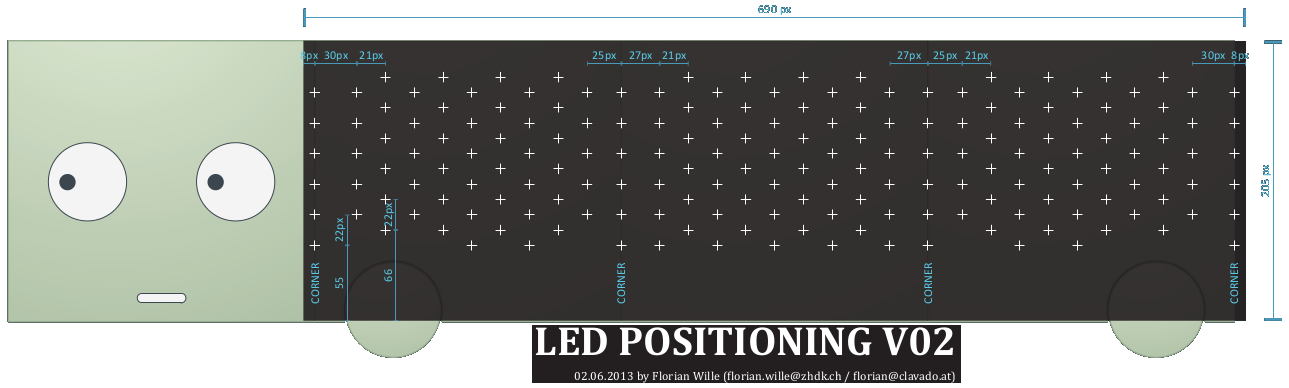
\includegraphics[width=14cm]{VideoSize.png}
    \caption{LED positionning for the creation of a video for the LEDs}
    \label{fig:VideoSize}
  \end{center}
\end{figure}

Once the video has been created, you simple need to open the robotWindow of the ranger (double click on the ranger model in Webots), and go to the tab called \textit{PatternGenerator}.\\

This utility allows you to chose the video, to specify if only the corner/face have to be taken into account or not, if you want to switch each LEDs off at the end and finally to reduce the number of frame. Once you have specify all the options, you can create the viedo file. The name of your file should be a number between 1 and 255 and have the extension "\textit{.vid}".\\

Finally you can add this new file on the SD card of the robot.\\

\section{Robot calibration (Outdated)}
\subsection{Neuil servos calibration}
In order to calibrate the servos of the eyes, go to the node \textit{neuil} of Aseba, first you have to update the array \textit{pos\_center} this array is used in order to define the center of the eye for the pupils. Therefore,  only the two first and two last components of this array are important (because the other are for the eyelid).\\

Then in order to adjust the interval of rotation of the eyelid, you have to update the arrays \textit{pos\_min} and \textit{pos\_max}. In order to do so, close and open the eyes at the maximum and update the corresponding values (this time it is the contrary, the two first and two last values are not important because the do not concern the eyelids).\\

Finaly, if the pupils move outside of the eyes or if in contrary the don't move enough, you can adjust the constant \textit{PUPIL\_RADIUS\_CONSTANT} (decreasing it will increase the maximum radius).\\ 

\subsection{TouchPanel calibration}
In order to calibrate the touch pannel, you have to find the good threshould for each touch sensors. In order to do so, put the program \textbf{TouchPanelCalibration.aesl} in the node RangerMain, then run it and touch carefully with the hand every part of the pannels (especially where touch sensors are located). Then emit the event \textit{ComputeThreshold}, the threshold for each sensors is then computed, by taking into account the minimum value encountered (when the hand is closest to the sensors) and the maximum value encountered (sensors do not see had at all).\\

The thresold values are now stored in the arrays \textit{touchLeftThreshold}, \textit{touchRearThreshold} and \textit{touchRightThreshold}, you just have now to copy these values in the same arrays of the main Aseba code.\\

\newpage
\section{Use the custom event}
If you need to use a custom event in order to add your custom code on one (or several) of the aseba nodes (for example to play specific pattern with the LEDs or game with the touchsensors) you can easily use the event \textit{customEvent}, this event has 10 arguments.\\

From the computer you can use the funtion \textit{emitCustomEvent} from the class DifferentialWheels:
\lstset{language=c++} 
\lstset{commentstyle=\textit} 
\begin{lstlisting} 
void emitCustomEvent(int *tab);
\end{lstlisting}
The function take as arguments a array of ten integers, which are the arguments emitted with the event.\\

\appendix

\chapter{Aseba Events}\label{sec:asebaEvents}
\begin{figure}[H]
\begin{center}
\begin{tabular}{|l|c|c|}
   \hline
   \textbf{event name} & \textbf{arguments} & \textbf{direction}\\
   \hline
   \hline
   mainFeedback & 16 & computer \textcolor{red}{<-} robot \\
   \hline
   mainFeedbackWithEncoders & 20 & computer \textcolor{red}{<-} robot \\
   \hline
   setLed & 3 & computer \textcolor{green}{->} robot \\
   \hline
   receiverFeedback & 10 & computer \textcolor{red}{<-} robot \\
   \hline
   setSpeed & 2 & computer \textcolor{green}{->} robot \\
   \hline
   enableEncoders & 1 & computer \textcolor{green}{->} robot \\
   \hline
   playLedVid & 2 & computer \textcolor{green}{->} robot \\
   \hline
   stopLedVid & 0 & computer \textcolor{green}{->} robot \\
   \hline
   neuilFeedback & 4 & computer \textcolor{red}{<-} robot \\
   \hline
   neuilEvent & 8 & computer \textcolor{green}{->} robot \\
   \hline
   customEvent & 10 & computer \textcolor{blue}{<->} robot \\
   \hline
   emitterEvent & 7 & computer \textcolor{green}{->} robot \\
   \hline
   enableFeedback & 1 & computer \textcolor{green}{->} robot \\
   \hline
\end{tabular}
\end{center}
\label{tab:event}
\caption{Events used by the aseba nodes.}
\end{figure}

\newpage
\chapter{Events map}\label{sec:eventsMap}
\begin{figure}[H]
  \begin{center}
    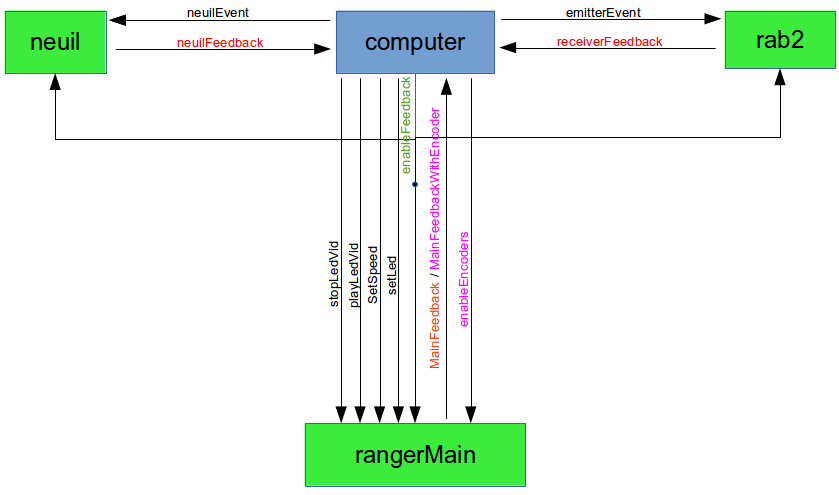
\includegraphics[width=14cm]{EventMap.png}
    \caption{Events map. Feedback (in red) from the various modules can be enable/disable by the event \textit{enableFeedback} (in green). Events from the various modules to the computer are used in order to transmit sensors state and events in the other direction (computer to modules) are used in order to give command to the actuators of each modules.}
    \label{fig:EventMap}
  \end{center}
\end{figure}

\end{document}
